\newpage
\section{SVM}
SVM sta per support vector machine ed è un classificatore derivato dalla teoria dell'apprendimento di Vpnik. Dopo anni
di sviluppi teorici, SVM divenne famosa quando, utilizzando le immagino come input, ha fornito una precisone paragonabile a reti neurali
SotA (negli anni 90) con funzionalità progettate a mano in un compito di riconoscimento della grafica. \\\\
Attualmente SVM è ampiamente utilizzato in tutti i campi di applicazione di apprendimento supervisionato, utilizzato anche per la regressione. Anche se le attuali deep-neural-network spesso 
li supra in molti ambiti (ad esempio analisi delle immagini).\\\\
Partimao dal modello lineare per la classificazione, ed ancora, siamo interessati anche ad arrichirlo per problemi non lineari.

\subsection{Maximum margin classifier}
Problema di classificazione binaria. Cominciamo ad assumerre un problema lineare separabile e assumiamo anche l'assenza di dati sul rumore (margine rigido del SVM).
\begin{example}
    Facciamo un esempio di margini. Infatti non tutti gli iperpiani che risolvono il compito sono uguali, variando l'iperpiano di sepazione varia anche il margine.
    \begin{figure}[h!]
        \centering 
        \begin{subfigure}{.25\textwidth}
            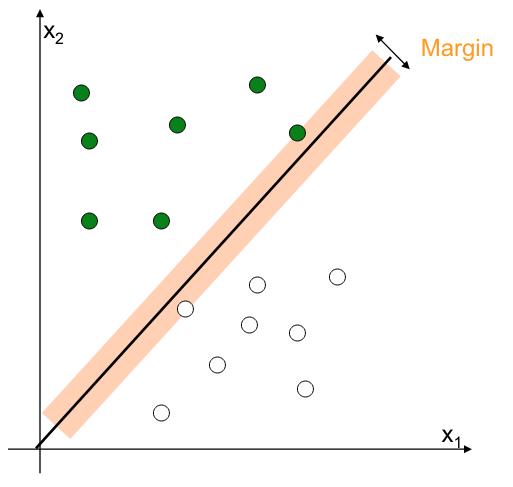
\includegraphics[width=1\textwidth]{images/esempio-margini-1.png}
        \end{subfigure}
        \begin{subfigure}{.30\textwidth}
            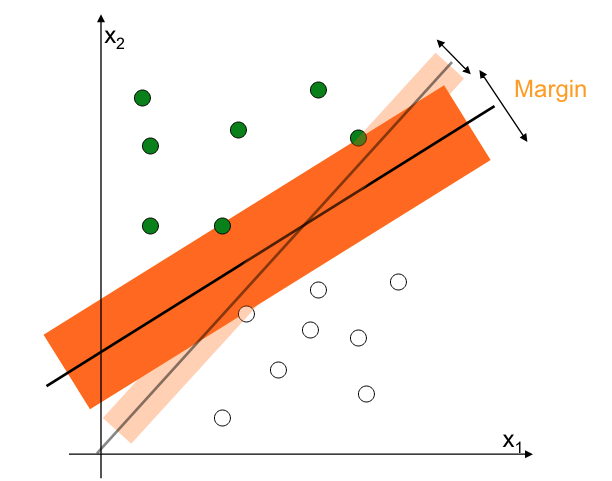
\includegraphics[width=1\textwidth]{images/esempio-margini-2.png}
        \end{subfigure}
        \begin{subfigure}{.43\textwidth}
            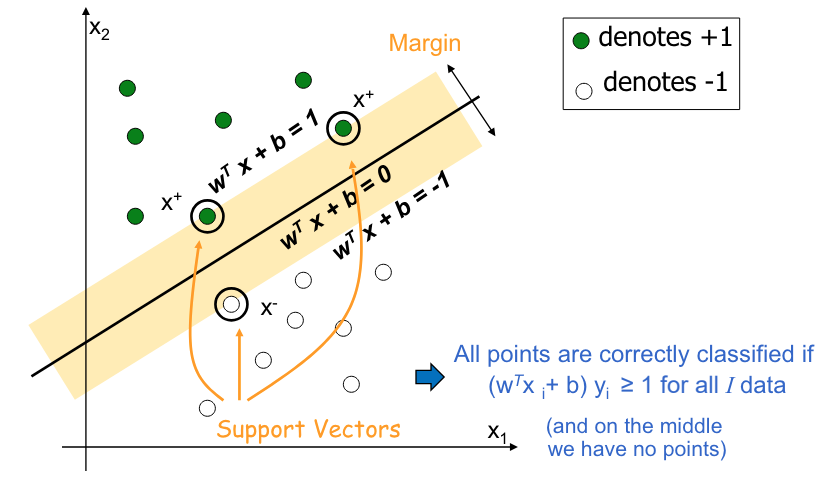
\includegraphics[width=1\textwidth]{images/esempio-margini-3.png}
        \end{subfigure}
    \end{figure}
\end{example}
\begin{definition}
    Il \textbf{margine} è (il doppio della) distanza tra l'iperpiano di separazione e i punti dati più vicini (esempi di input).
\end{definition}
\begin{definition}
    Definiamo anche \textbf{vettori di supporto}
    $$x_p \:\: t.c. \:\: |w^T x_p + b| = 1 \hspace{15pt} b = w_0$$
\end{definition}
Consideriamo il problema di apprendere un modello lineare per la classificazione binaria, cioè una fuzione nella forma
$h: \mathbb{R}^n \to \{-1, 1\}$, come per esempio $h(x) = sign(wx + b)$, sulla base di esempi $(x_p, y_p)$ nel TR set.
\begin{definition}
    Definiamo \textbf{training problem} come trovare $(w, b)$ tale che tutti i punti siano classificati correttamente e il 
    margine è massimizzato.
\end{definition}
\hspace{-15pt}Un vincolo è che:
$$(w^T x_p + b) y_p \geq 1 \: \forall p$$
Che vuol dire che \textbf{tutti i punti sono correttamente classificati}. Si noti inoltre che, a differenza della soluzione LMS,
per i casi separabili linearmente qui abbiamo 0 errori.